\documentclass[UTF-8, a4paper, 12pt]{ctexart}

\usepackage[left=1in,right=1in,top=1.00in,bottom=1.00in]{geometry}
\usepackage[colorlinks,linkcolor=blue,anchorcolor=blue,citecolor=green,CJKbookmarks=True]{hyperref}
\usepackage{CJK,CJKnumb}
%\usepackage{indentfirst}        % 首行缩进宏包
%\usepackage{latexsym,bm}        % 处理数学公式中和黑斜体的宏包
\usepackage{amsmath,amssymb}     % AMSLaTeX宏包 用来排出更加漂亮的公式
\usepackage{graphicx}
\usepackage{cases}
\usepackage{pifont}
\usepackage{txfonts}
\usepackage{subfigure}
\usepackage{pdfpages}
\usepackage{listings}
\usepackage{xcolor}
\usepackage[subfigure]{tocloft}     % 模板中用了subfigure,不加此选项会产生冲突

\CTEXsetup[format={\Large\bfseries}]{section}
\zihao{-4}\linespread{1.5}\selectfont
\renewcommand{\theequation}{\arabic{section}-\arabic{equation}}
\renewcommand{\thefigure}{\arabic{section}-\arabic{figure}}
%\renewcommand{\thefigure}{\thechapter-\arabic{figure}}


\renewcommand{\cftsecleader}{\cftdotfill{\cftdotsep}}

\renewcommand\contentsname{{\qquad\qquad\qquad\qquad\qquad\qquad 目\quad 录}}


\newcommand{\song}{\CJKfamily{song}}    % 宋体   (Windows自带simsun.ttf)




\title{\bfseries \Huge  利用汇编语言计算字符串CRC-32校验和}
\author{1120183150 胡森康}
\date{\today}





\begin{document}
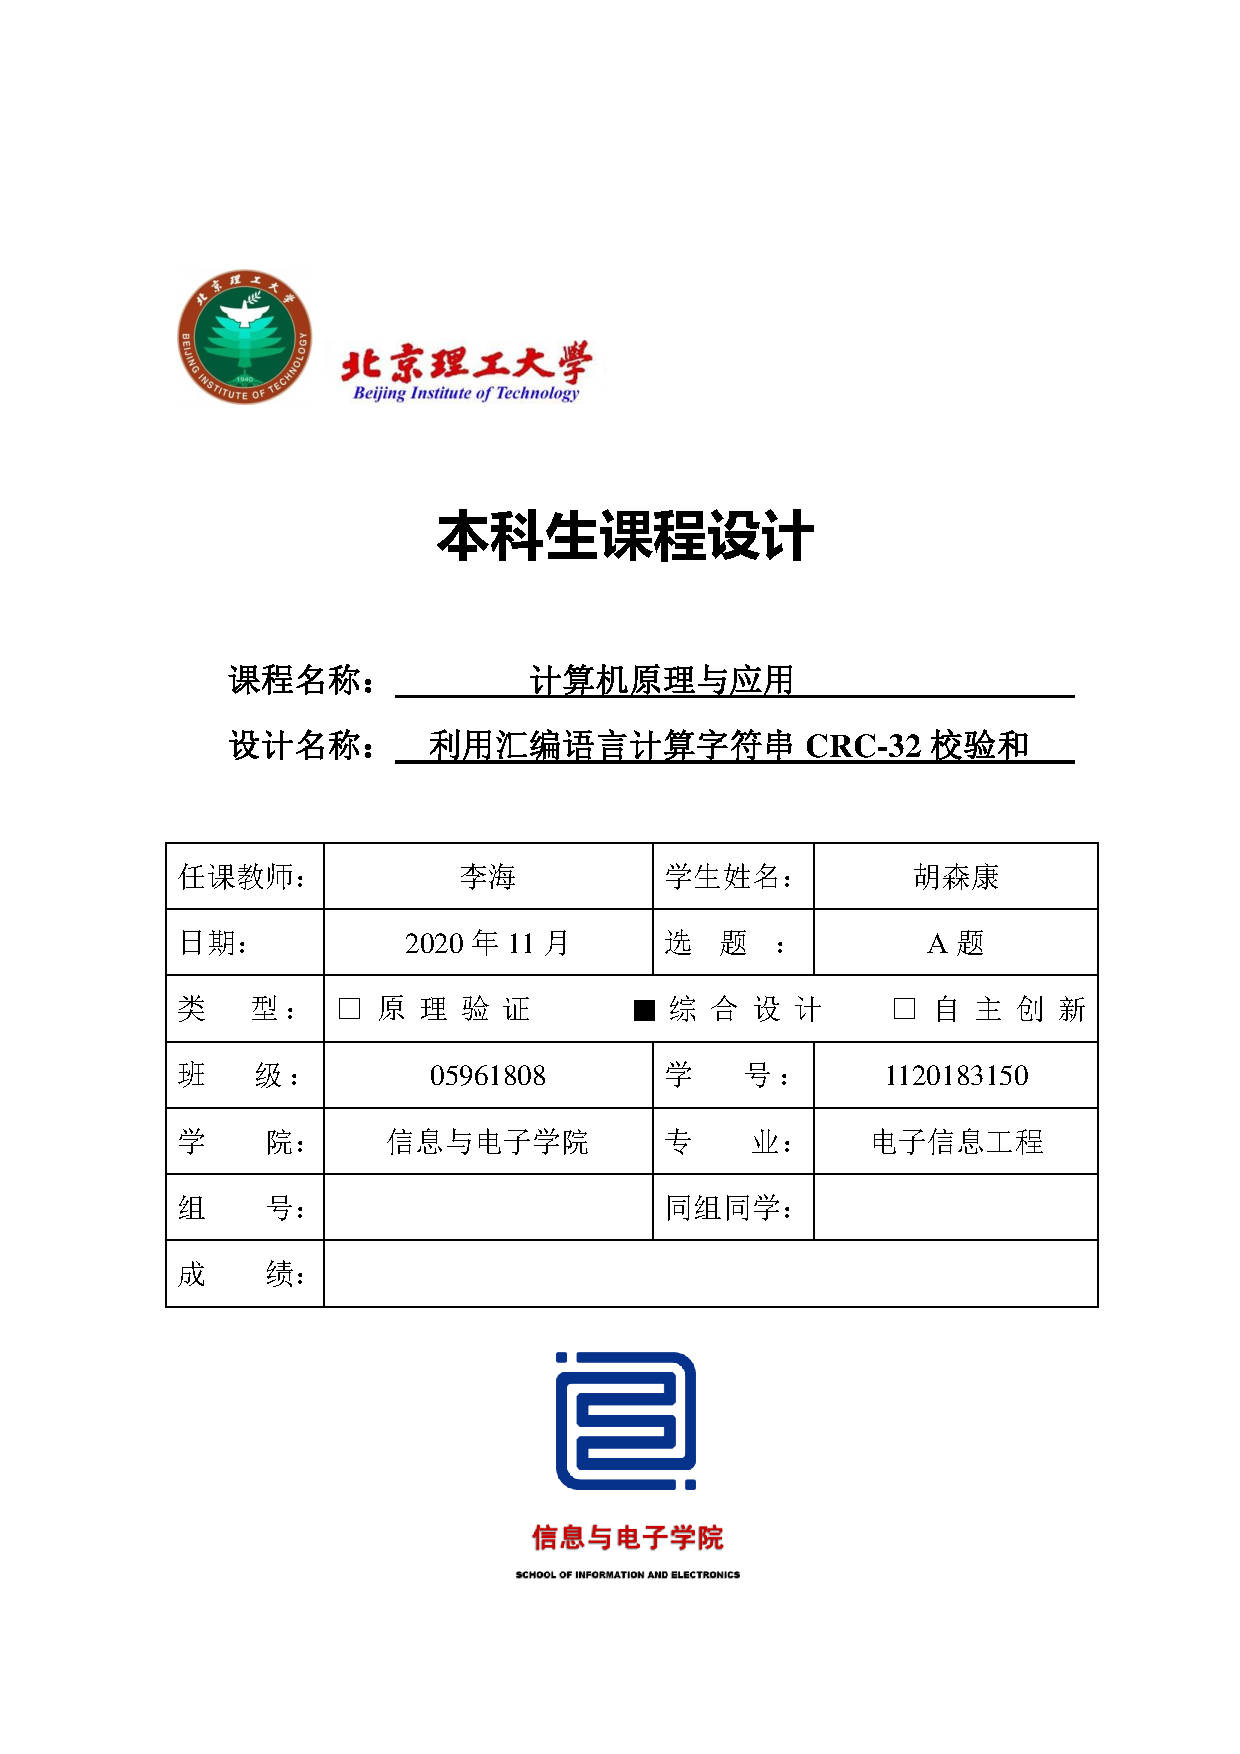
\includepdf[pages={1}]{coverpage.pdf}


\thispagestyle{empty}
\newpage
\thispagestyle{empty}

\maketitle
\tableofcontents
\newpage

\section{实验任务}
\begin{itemize}
    \item 在程序时间段定义一个字符串用于测试CRC-32 校验和的计算;
    \item 编写子程序计算CRC-32 校验和,生成多项式为:
    $x^{32}+x^{26}+x^{23}+x^{22}+x^{16}+x^{12}+x^{11}+x^{10}+x^{8}+x^{7}+x^{5}+x^{4}+x^{2}+x+1$
    \item 主程序调用子程序计算校验和后,将结果输出到屏幕。
\end{itemize}
\section{实验环境}
    \begin{itemize}
        \item VSCODE
        \item MASM插件(16位环境)
    \end{itemize}
\section{理论原理}
循环冗余校验(英语:Cyclic redundancy check,通称“CRC”)
是一种根据网络数据包或电脑文件等数据产生简短固定位数校验码的一
种散列函数,主要用来检测或校验数据传输或者保存后可能出现的错误。
生成的数字在传输或者存储之前计算出来并且附加到数据后面,然后接收
方进行检验确定数据是否发生变化。由于本函数易于用二进制的电脑硬件
使用、容易进行数学分析并且尤其善于检测传输通道干扰引起的错误,因
此获得广泛应用。

采用CRC校验时,发送方和接受方用同一个生成多项式$g(x)$, $g(x)$ 是一个 $GF(2)$ 多项式,并且 $g(x)$ 的首位和最后一位的系数必须为 1 。

CRC的处理方法:发送方用发送数据的二进制多项式$t(x)$除以$g(x)$,得到余数$y(x)$作为CRC校验码。校验时,以计算的矫正结果是否为0为据,判断数据帧是否出错。设生成多项式是$r$阶的,(最高位为$x^r$)具体步骤如下:
\begin{enumerate}
    \item 在发送的 m 位数据的二进制多项式 $t(x)$后添加 $r$个 0 ,扩张到 $m+r$位,以容纳 $r$ 位的校验码,追加 0 后的二进制多项式为  $T(x)$ 
    \item 用生成多项式$g(x)$除以$T(x)$,得到$r$位余数$y(x)$,它就是CRC校验码。
    \item 把 $y(x)$ 追加到 $t(x)$ 后面,此时的数据 $s(x)$ 就是包含了 CRC 校验码的待发送字符串;由于 $s(x) = t(x) y(x)$ ,因此 $s(x)$ 肯定能被 $g(x)$ 除尽。
    
\end{enumerate}

\section{算法思路}


CRC-32码由四个字节构成,在开始时CRC寄存器的每一位都预置为1,
然后把CRC寄存器与8bit的数据进行异或,之后对CRC寄存器从高位
到低位进行移位,在最高位的位置(MSB)补0,而最低位(LSB,移
位后已经被移出CRC寄存器)如果为1,则把寄存器与预定义的多项式
码进行异或,若LSB为0,则无需进行异或。重复上述的由高至低的
移位8次,第一个8bit数据处理完毕,用此时CRC寄存器的值与
下一个8bit数据异或并进行如前一个数据似的8次移位。所有字符处
理完成后CRC寄存器内的值即为最终的CRC值。

具体过程如下:
\begin{enumerate}
    \item 设置CRC寄存器,并给其赋值FFFFH
    \item 将数据的第一个8bit字符与32位CRC寄存器的低8位进行异或,
    并把结果存入 CRC 寄存器。
    \item CRC寄存器向右移移位,MSB补0,移出并检查LSB。
    \item 重复第3与第4步直到8次移位全部完成,此时一个8bit数据处理完毕。
    \item 重复2至5步直到所有数据全部处理完毕。
    \item 最终CRC寄存器的内容即为CRC值。
\end{enumerate}


\section{程序介绍}

本程序的代码段由4个程序组成,分别是主程序$main$
,CRC校验和计算子程序$calculate\_CRC$,二进制结果输出子程序$output\_BIN$
和十六进制结果输出子程序$output\_HEX$组成。

当用户输入一串字符时,计算其CRC-32校验和并分别将其输出为二进制数和
十六进制数,当用户输入字符“$\#$”时,程序结束。

\subsection{CRC校验和计算子程序}
CRC校验和计算子程序如下图(\ref{1})所示
\begin{figure}[htbp]
    \centering
    
\includegraphics[height=15cm]{fig/f1.png}
    \caption{CRC校验和计算子程序流程图}
    \label{1}
\end{figure}

\subsection{二进制结果输出子程序}
二进制输出的主要思路为:对寄存器中的数进行左移,使最高位溢出到标志位$CF$中,
再利用有符号加法$adc$将$CF$中的值取出,并输出即可。

流程图如下图(\ref{bin})所示:
\begin{figure}[htbp]
    \centering
    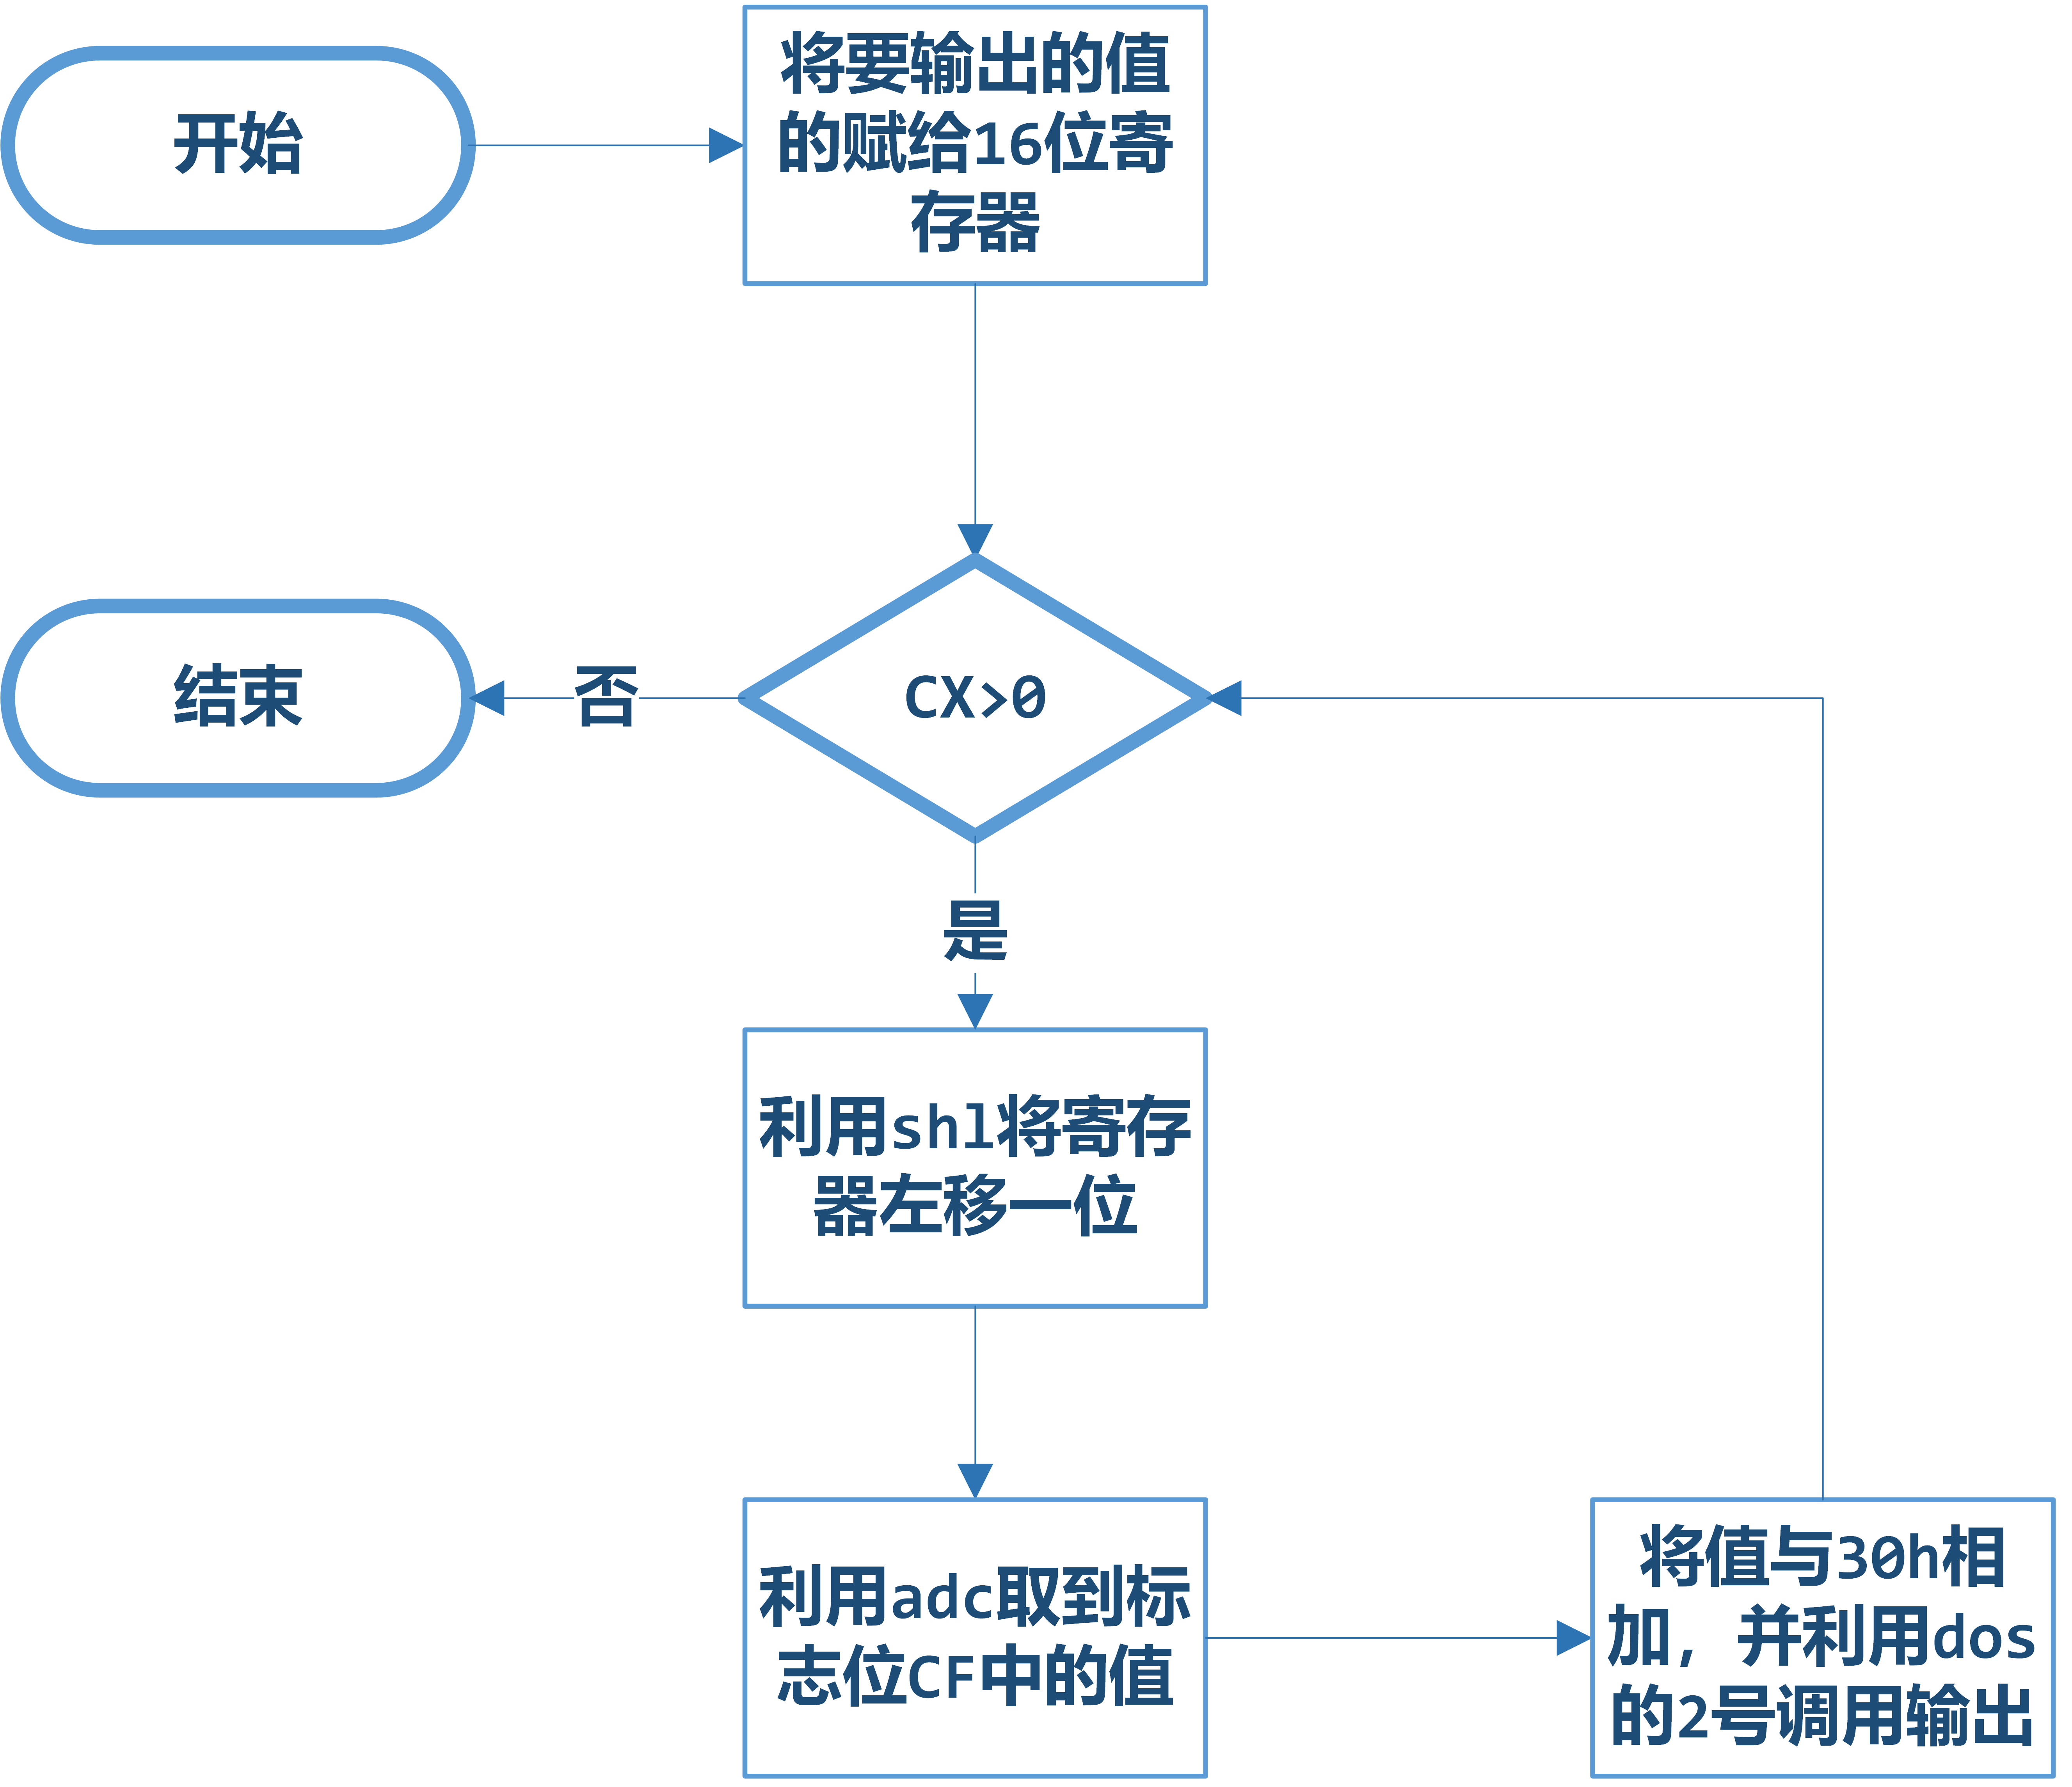
\includegraphics[width=10cm]{fig/f5.png}
    \caption{二进制结果输出子程序流程图}
    \label{bin}
\end{figure}

\subsection{十六进制结果输出子程序}
十六进制输出的主要思路为:先考虑高八位,使八位数据逻辑右移四位,再加上30h,
比较是否是对应字符的ASCII码,即是否小于39h,小于则可以直接输出,
因为此时对应的就是该数字的ASCII码;
用高八位与0fh做与运算,使高四位为0,低四位为原来的数值,再与30h相加,比较是否小于39h,小于则直接输出,
若大于39h,则表示要输出的是A-F,将其自加7h,得到正确的ASCII码,然后输出。

流程图如下图(\ref{hex})所示:
\begin{figure}[htbp]
    \centering
    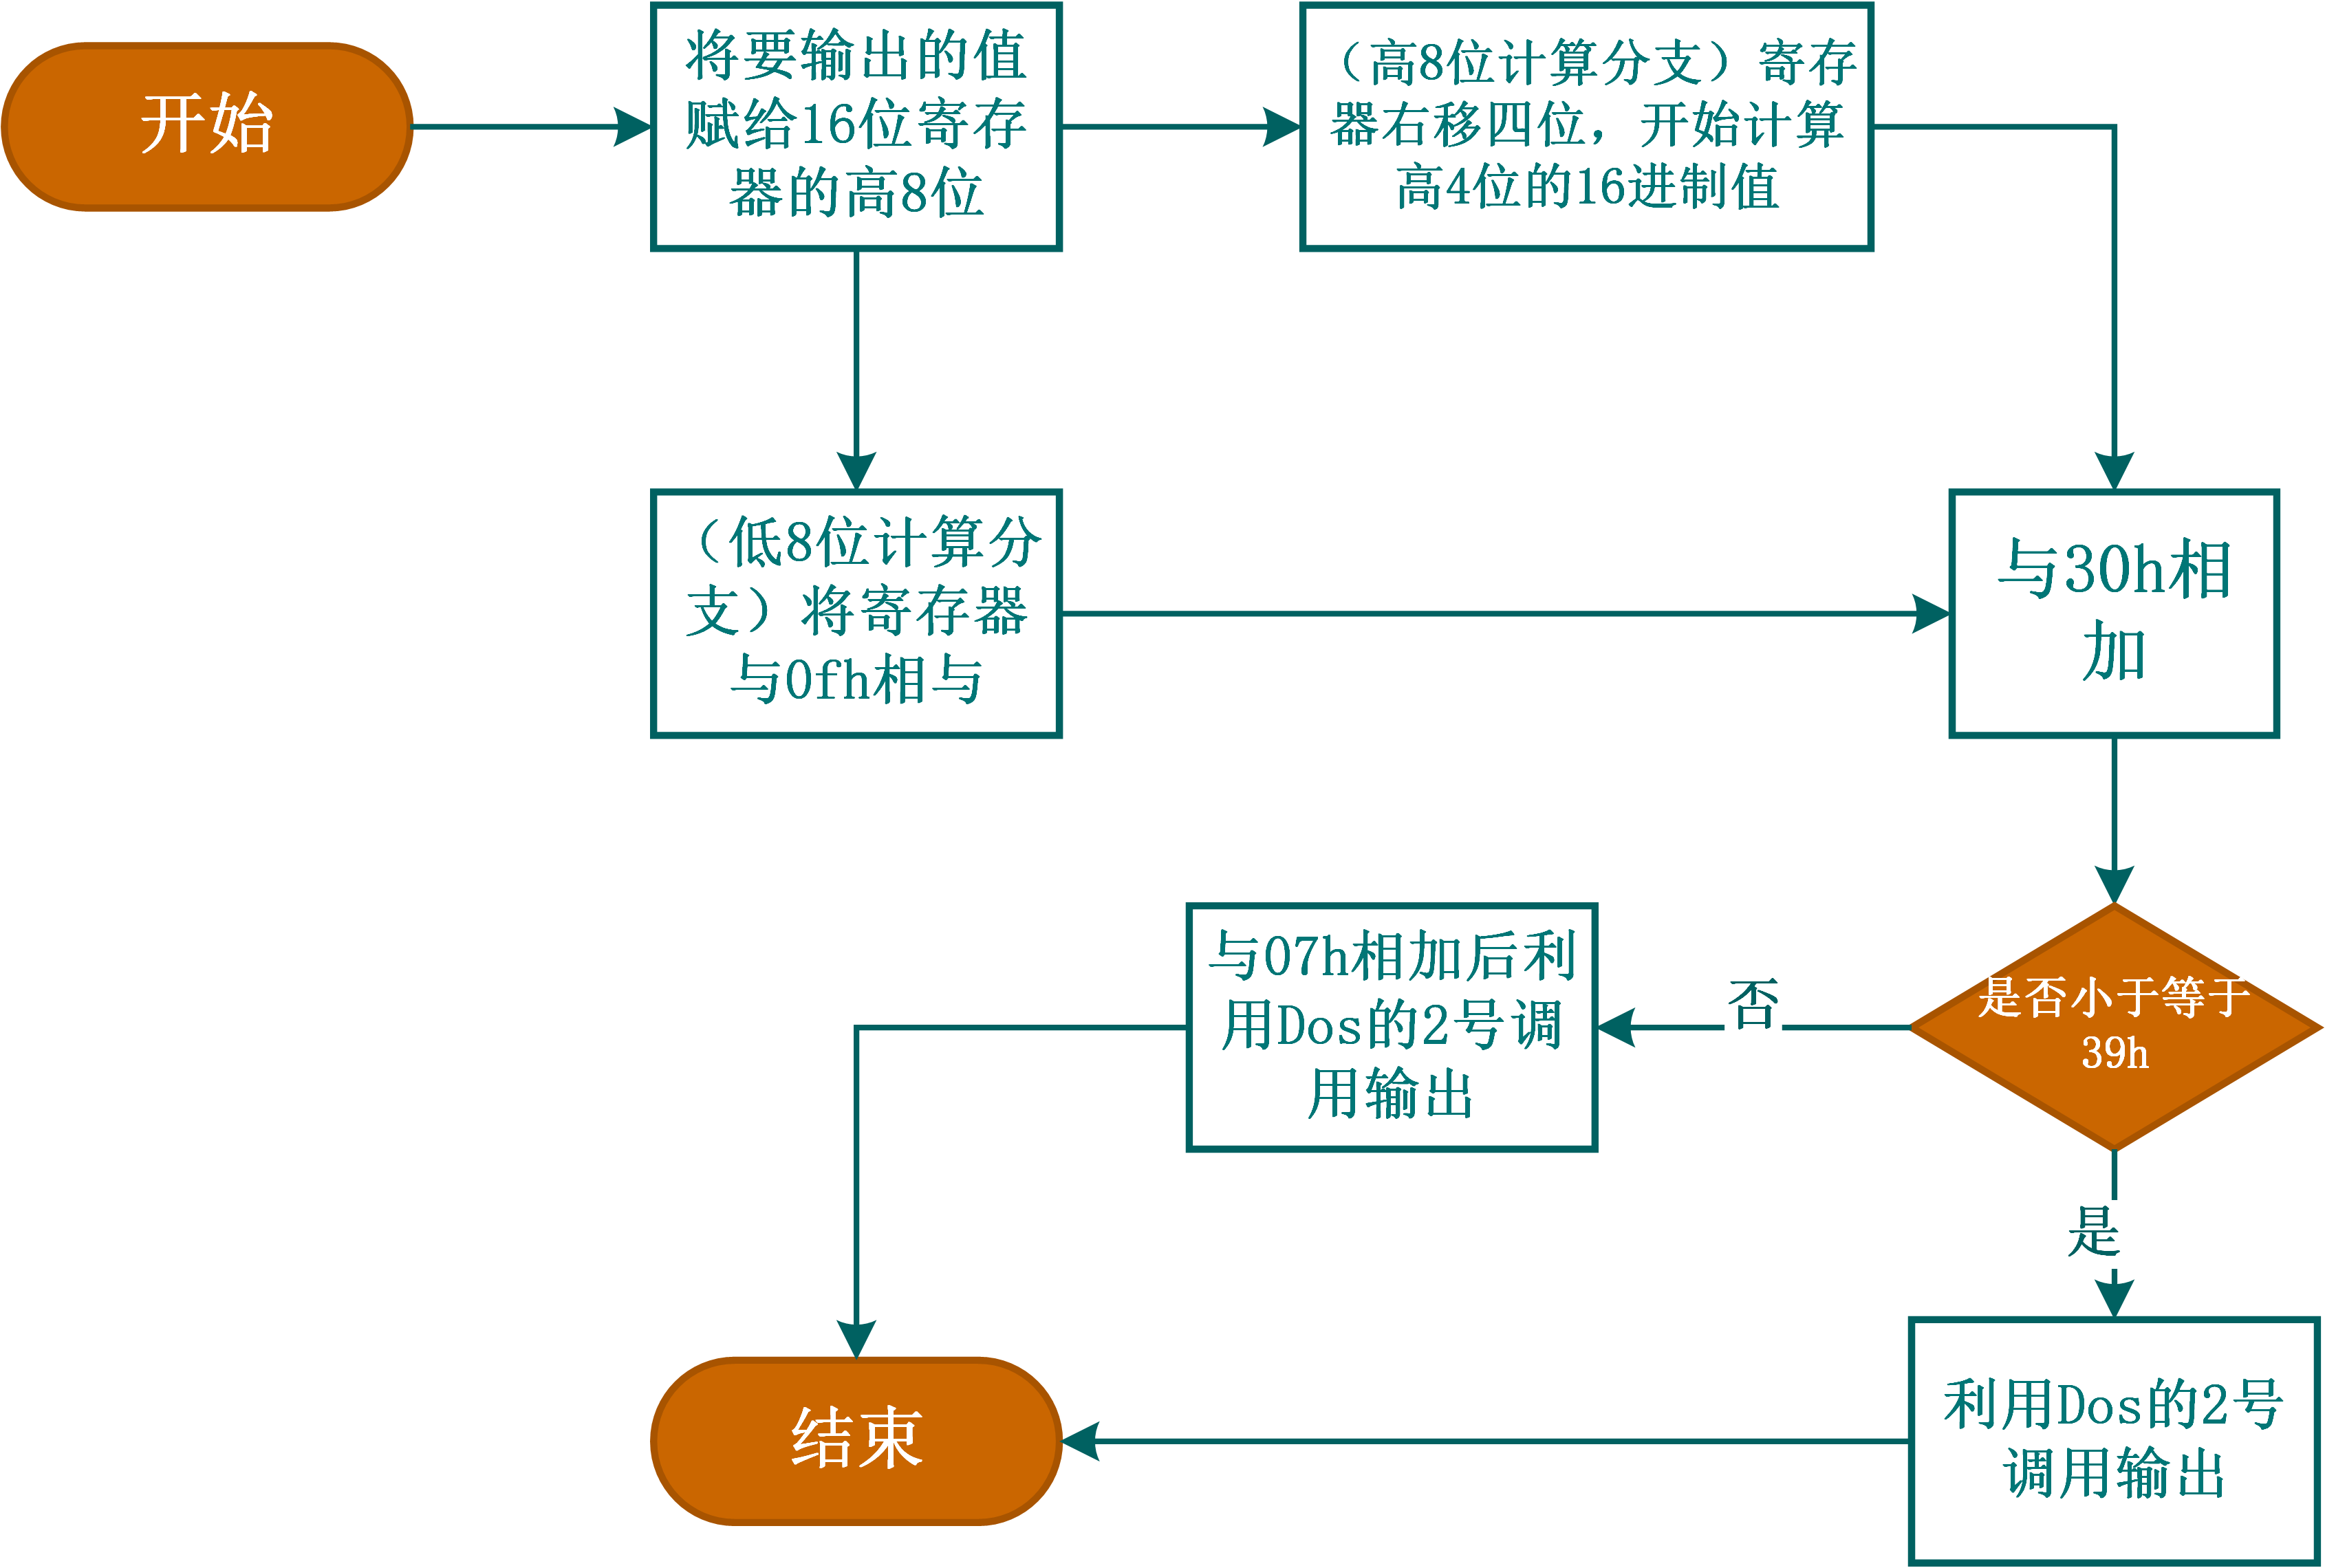
\includegraphics[width=10cm]{fig/f6.png}
    \caption{十六进制结果输出子程序流程图}
    \label{hex}
\end{figure}



\newpage

\section{程序结果}
程序运行结果如下图(\ref{2})所示:
\begin{figure}[htbp]
    \centering
    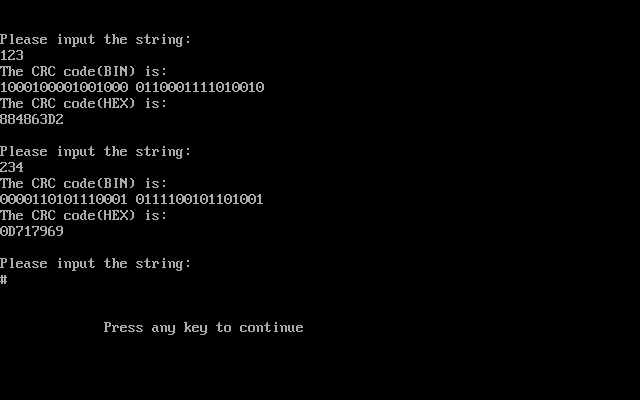
\includegraphics[width=12cm]{fig/f2}
    \caption{程序运行结果}
    \label{2}
\end{figure}

可见,输入字符串为123时,程序输出的CRC-32二进制校验码为1000\ 1000\ 0100\ 1000\ 0110\ 0011\ 1101\ 0010,
十六进制校验码为884863d3h,经检验是正确的。

此时,程序并没有退出,而是继续等待用户输入字符串。用户输入字符串为234时,
程序输出的CRC-32二进制校验码为
0000\ 1101\ 0111\ 0001\ 0111\ 1001\ 0110\ 1001,十六进制校验
码为0d717969h,经检验是正确的。

当用户继续输入一个$\#$时,程序结束。
\newline

更多的结果如下:

\begin{figure}[htbp]
    \centering
    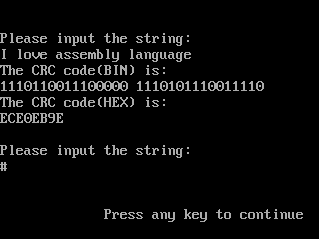
\includegraphics[width=6cm]{fig/f4.png}
    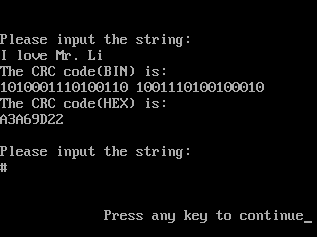
\includegraphics[width=6cm]{fig/f3.png}
\end{figure}


\section{思考题}
\subsection{题目描述}
是否有2个字符串的CRC-32校验和是相同的?
\subsection{解答}

可能有两个字符串的CRC-32校验和是相同的。

对于32位校验,若输入超过32位,因此不能有超过$2^{32}$个不同的输入来
生成不同的CRC。
且CRC多项式是线性结构,可以很容易地故意改变数据而维持CRC不变。

就比如字符串“b5a7b602ab754d7ab30fb42c4fb28d82”
和字符串\newline “d19f2e9e82d14b96be4fa12b8a27ee9f”的CRC-32就是相同的,均为997d37bah
如下图(\ref{same})所示:

\begin{figure}[htbp]
    \begin{center}
        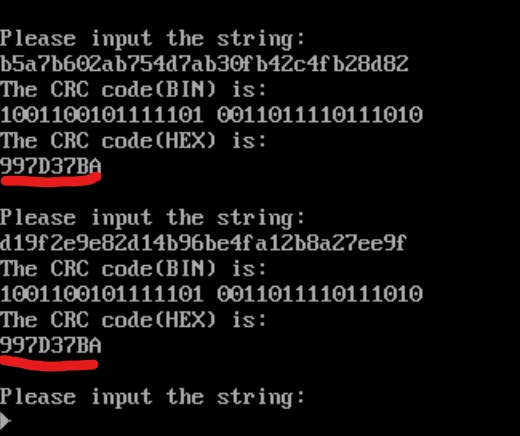
\includegraphics[width=6cm]{fig/ff.jpg}
    \end{center}
    \caption{CRC-32相同的两个字符串}
    \label{same}
\end{figure}
\section{收获和感想}

在本次大作业中我收获了很多,首先是自学的能力,其次是编程的能力。

在进行大作业的过程中,我看了一些文献和博客,将CRC校验的原理搞清,并思考实现的算法。在这个过程中
增强了我的自主学习能力,也收获了很多新的知识,比如模2除的计算方法。
搞清楚了CRC校验的原理,接下来就是如何计算CRC码,这就涉及到了算法的问题了,在思考算法的过程中,
我意识到模2除的本质是异或。因此很快便明确了算法的方向,就是不断的移位和异或。

因为是32位校验,因此在编程的过程中我先利用了vs进行编程,算法很简洁,也是正确的,但编出来总是结果不正确,这个
问题让我头疼了好几天,最终还是在李老师的点播下才成功。在32位环境中是比较好实现,但不知道什么问题我的vs
总是导不进masm的库,这就导致了我不能使用stdout等函数进行输入输出,我看了很多技术帖子,但还是
没解决我的vs谜之一样的bug,遂放弃用vs编,改用vscode的masm插件(16位)。虽然利用16位环境算法
稍稍比32位环境复杂点,但还是很快就将32位代码移植到16位环境中了。

在保证程序能得到正确的结果后,便开始处理输入和输出,主要是输出。要将结果输出为2进制或16进制也是需要一些代码量的,
在处理输入输出的过程中虽然也遇到了很多意想不到的bug,但还是被成功解决了。

在此次大作业中,我意识到要熟练掌握编程,核心在于多动手去编。其次是,数学原理和算法
很多时候差别是很大的,比如计算CRC,数学原理是对进行模2除,最后得到余数即为结果,但在算法中
是进行移位和异或,这在表面上是不同的,而且此种情况在低级语言中由显得突出,因为这和芯片的运作方式是分不开的。


\end{document}